%% Bridging Pre- and Post-Silicon Stimulus Generation for RISC-V Debug
%% DVCon Europe / IEEE conference format.
\documentclass[conference]{IEEEtran}
\IEEEoverridecommandlockouts
\usepackage{cite}
\usepackage{amsmath,amssymb,amsfonts}
\usepackage{algorithmic}
\usepackage{graphicx}
\usepackage{textcomp}
\usepackage{xcolor}
\usepackage{booktabs}
\usepackage{tabularx}
\usepackage[hidelinks]{hyperref}
\usepackage{url}
\def\BibTeX{{\rm B\kern-.05em{\sc i\kern-.025em b}\kern-.08emT\kern-.1667em\lower.7ex\hbox{E}\kern-.125emX}}

\begin{document}

\title{Bridging Pre- and Post-Silicon Stimulus Generation for RISC-V Debug\\
{\large A Python-Based Cross-Platform Framework}}

\author{
\IEEEauthorblockN{Jahanzeb Khalid}
\IEEEauthorblockA{\textit{10xEngineers} \\
Lahore, Pakistan \\
jahanzeb.khalid@10xengineers.ai}
\and
\IEEEauthorblockN{Hassan Ashraf}
\IEEEauthorblockA{\textit{10xEngineers} \\
Lahore, Pakistan \\
hassan.ashraf@10xengineers.ai}
}

\maketitle

\begin{abstract}
Verifying a RISC-V Debug Module is split across two disciplines that share almost no artifacts. Pre-silicon teams write SystemVerilog/UVM sequences against the Debug Module Interface (DMI); post-silicon teams drive the same hardware through OpenOCD or GDB over JTAG. The result is duplicated effort, divergent coverage, and a reproduction gap: a debug test that fails on a lab bench cannot be replayed in the simulation environment without a human re-encoding it by hand. This paper presents a Python framework that closes that gap by decoupling a debug test's \textit{intent} from its \textit{transport}. One command layer expresses the scenario; one abstract transport interface reaches either a UVM testbench, through a socket and DPI-C bridge, or physical silicon, through OpenOCD over JTAG, with the stimulus unchanged. We evaluate on two RISC-V cores --- CVA6 with a specification-v1.0 debug module, and Ibex with an unmodified v0.13 module --- running 17 specification-traceable scenarios per core, each self-checked against a SystemVerilog reference model derived from the specification text rather than from the RTL. Both reach 100.00\% merged functional coverage over 14 covergroups. All 17 stimulus files then execute unmodified on an Arty A7 FPGA board: measured across every scenario, the entire per-target delta is declarative configuration, and the stimulus layer contains no transport-conditional logic in 2259 lines. The complete SystemVerilog surface the framework requires is 120 lines, written once and unchanged as the scenario count grew to 17. We also quantify what portability costs: routing through OpenOCD's Remote Bit-Bang path is 2.5--103$\times$ slower than the direct bridge, and that multiplier tracks how thin the direct path already is rather than being a fixed tax. We position the work against the Accellera Portable Stimulus Standard and the classical transactor pattern, claiming novelty not in transaction abstraction but in a debug-protocol-specific transport seam spanning the pre/post-silicon boundary.
\end{abstract}

\begin{IEEEkeywords}
RISC-V; Debug Module; functional verification; UVM; Python; JTAG; OpenOCD; portable stimulus; functional coverage.
\end{IEEEkeywords}

\section{Introduction}
Modern System-on-Chip verification is characterised by the ``shift-left'' paradigm, in which teams run software and system-level tests as early as possible. Hardware debug infrastructure, and specifically the RISC-V Debug Module \cite{b1}, resists this paradigm because of a structural divide in how pre-silicon and post-silicon teams work.

Pre-silicon verification of the Debug Module is typically performed with constrained-random UVM sequences. These verify DMI bus protocol compliance and corner-case timing well, but capture the high-level, stateful workflows of a real debugger poorly. A debugger executes long, state-dependent sequences: halting a hart, issuing abstract commands to read General Purpose Registers, writing instructions into the program buffer, stepping the program counter. Expressing these purely in SystemVerilog is verbose and binds the tests to one verification environment.

Post-silicon validation, conversely, relies on software tools such as OpenOCD communicating over physical JTAG. When a debug test fails on the lab bench, root-causing it is hard, because the hardware stimulus --- the exact sequence of JTAG shifts --- cannot be replayed natively in the UVM environment. Engineers translate debug logs into SystemVerilog sequences by hand to reproduce bugs in RTL, which is slow and error-prone. The two artifacts then drift.

This paper closes that gap by decoupling the \textit{intent} of a debug test --- which registers to access, which assertions to make --- from the \textit{transport}, the medium used to reach the chip. Our contributions are: (1) a debug-protocol-specific transport seam that reaches a UVM simulation and physical silicon from one unmodified stimulus artifact, measured rather than asserted (Section IV-D); (2) a specification-derived reference model shared by both transports, so a hardware run is self-checked by the same predictor as a simulation run; (3) a cross-DUT differential diagnostic that localises a defect to verification code or design before any waveform is opened, with its limits characterised (Section IV-E); and (4) a measurement showing that Remote Bit-Bang transport overhead scales inversely with how thin the direct simulation path already is (Section IV-F).

\section{Related Work}
Table I compares this framework against the real alternatives for producing RISC-V debug stimulus.

\begin{table*}[!t]
\caption{Debug stimulus generation approaches compared}
\label{tab:I}
\centering
\footnotesize
\begin{tabular}{p{0.17\textwidth}p{0.16\textwidth}p{0.13\textwidth}p{0.42\textwidth}}
\toprule
Approach & Cross-platform reuse & Tooling cost & Closes the silicon-reproduction gap? \\
\midrule
Raw SystemVerilog/UVM sequences & None --- pre-silicon only & Simulator licence & No --- each scenario needs a hand-written OpenOCD equivalent for hardware \\
Random debug-stimulus generation \cite{b2} & None --- pre-silicon only & Generator + simulator & No --- targets simulation depth, not hardware reuse \\
OpenOCD native TCL scripting & None --- post-silicon only & Free & No --- the reverse problem; no path back into a UVM testbench \\
Manual translation of a bench failure into a SystemVerilog sequence & Not applicable --- a process, not an artifact & Engineer time & Nominally, but slow and error-prone by construction \\
Portable Stimulus Standard (PSS) \cite{b3} & High, at the scenario level, not the transport level & Often commercial tooling & Partially --- no native transport concept; needs a custom backend \\
\textbf{This framework} & \textbf{Full --- the same file, unmodified} & \textbf{Open-source only} & \textbf{Yes --- the sequence that failed on silicon is the reproduction script} \\
\bottomrule
\end{tabular}
\end{table*}

\textbf{Prior work on RISC-V debug verification.} The closest published work is Mishra \textit{et al.} \cite{b2}, who verify the debug unit of a RISC-V core by augmenting a biased-random assembly generator to emit debug sessions inside a running instruction stream, checked against a functional model. That work and this one are complementary and address different axes. Theirs maximises \textit{stimulus depth and randomness} within a simulation environment --- random instruction mixes, asynchronous debug requests, interrupts and bus faults interleaved --- which this framework does not attempt. Ours maximises \textit{execution-target portability} for a directed, specification-traced scenario set, and reaches hardware, which theirs does not address. A productive combination would use random generation of the kind in \cite{b2} above the transport seam described here.

\textbf{Python in verification.} Driving an HDL simulator from Python is established practice: cocotb \cite{b4} provides a coroutine-based cosimulation environment, and Hua \textit{et al.} \cite{b5} pair Python with UVM for memory-controller verification. This framework differs from both not in using Python, but in what sits below the API: cocotb and \cite{b5} terminate at a simulator, whereas the transport interface here also terminates at a physical chip.

\subsection{Relation to the Portable Stimulus Standard}
PSS \cite{b3} and this framework solve related but distinct problems, and the distinction is best stated as a difference of axis. PSS provides a declarative action and activity graph over a resource model, solved by a constraint engine to generate scenario \textit{variants}; its axis of power is scenario-space exploration, and realisation on a target is delegated to generated \texttt{exec} blocks. This framework provides an imperative stimulus library over a transport seam; its axis of power is execution-target portability, and scenario selection is directed and traceable rather than solved.

They share a goal --- separating what a test means from how it is realised --- and both aim at vertical reuse. They differ in abstraction level (declarative graph versus imperative call sequence), in generation model (constraint solving versus directed derivation from a specification-traced test plan), and decisively in that \textbf{PSS has no native concept of transport}: nothing in the standard models a JTAG, OpenOCD, or DPI-C path, so a PSS flow targeting both a UVM testbench and a physical board still requires exactly the execution backend this paper describes.

PSS is the better choice when the problem is combinatorial coverage of a large resource model, when scenarios must port across abstraction levels rather than across transports, and where its tooling is already licensed. This framework is the better choice when the protocol is narrow and deeply stateful --- the debug register space is small but its causal chains are long --- when zero tooling cost matters, and when the same engineers must read the stimulus on both sides of tape-out. The two compose naturally: a PSS \texttt{exec} block could target this framework's transport layer, letting PSS generate the activity graph while the seam here executes it against either target. We regard that as the most promising extension of this work rather than as a competing claim.

\subsection{Relation to the Transactor Pattern}
The architecture described in Section III is, at the transaction level, a transactor in the classical sense \cite{b6}: a high-level call is converted into bus-level activity by a component that hides the conversion. We claim no novelty for that mechanism, and any framework of this shape must implement it.

The distinction we do claim is one of scope. A classical transactor is compiled into a single execution environment and converts calls for the DUT it is built against; supporting a second target means writing a second transactor by hand, and the two then require synchronised maintenance. Here the transport interface has two implementations --- one reaching a UVM sequencer through DPI-C, one reaching a physical chip through OpenOCD --- selected at run time by configuration, with the stimulus above the seam byte-identical across both. Section IV-D measures that identity rather than asserting it: across 17 scenarios the stimulus layer contains no transport-conditional logic of any kind, and the whole per-target difference is declarative.

Two consequences follow that a single-environment transactor does not provide. First, the reference model that checks a simulation run also checks the hardware run, because it sits above the seam. Second, because the same stimulus reaches two dissimilar DUTs, the \textit{distribution} of a failure across them carries diagnostic information (Section IV-E). Neither is a property of transaction abstraction as such; both follow from placing the seam at the pre/post-silicon boundary for a protocol whose two toolchains are normally maintained by different teams.

Beyond the seam, the choice of Python over TCL --- the incumbent on the post-silicon side --- supplies real control flow, exceptions, and type annotations, and gives the stimulus direct access to an existing test and CI ecosystem, so a scenario regresses nightly against both a simulator and a lab board without a bespoke harness.

\section{Methodology}
Figure 1 shows the architecture. A single Python stimulus, expressed once against the \texttt{RISCVDebug} command API, reaches either target through one abstract \texttt{DebugTransport} interface; only the branch beneath that interface differs.

\begin{figure}[!t]
\centering
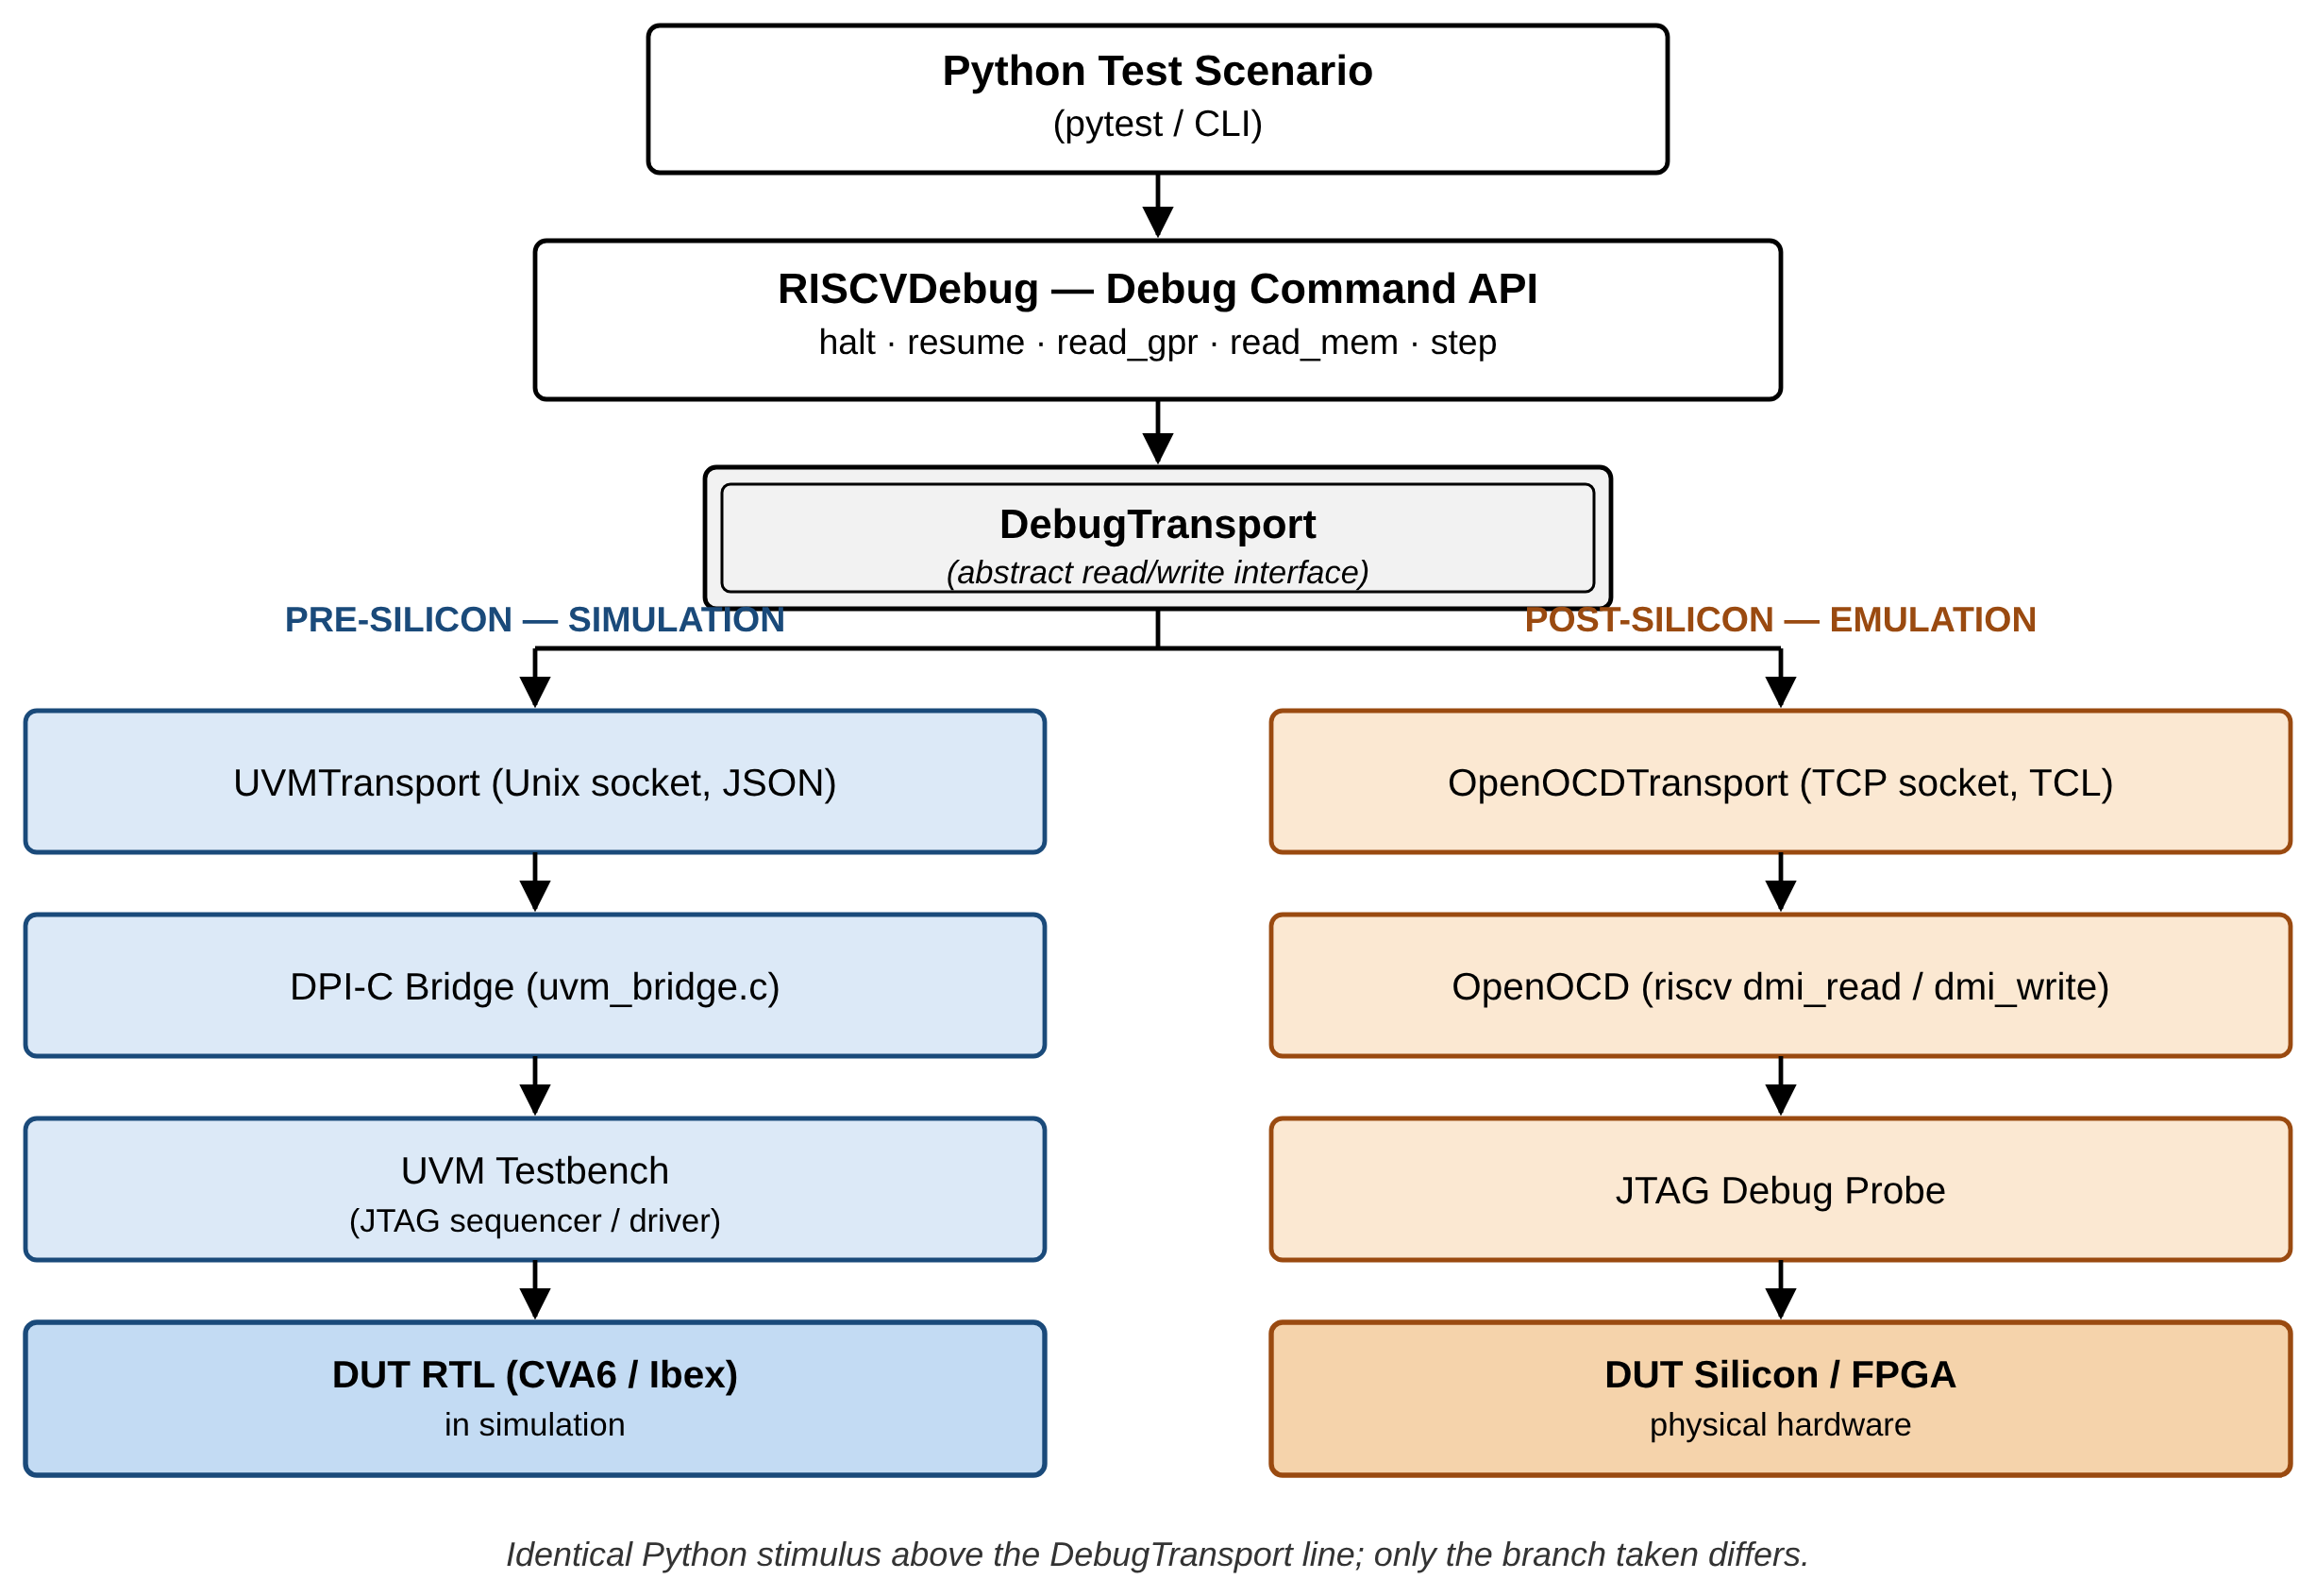
\includegraphics[width=\columnwidth]{figures/figure1_architecture}
\caption{Unified dual-transport architecture: identical Python stimulus above the \texttt{DebugTransport} interface reaches a UVM simulation (left) or physical silicon (right) unmodified.}
\label{fig:1}
\end{figure}

\subsection{Python Orchestration Layer}
Scenarios are written against a fluent API modelling the RISC-V debugger. Each is a debug session of ordered steps; a halt scenario writes 1 to \texttt{dmcontrol.haltreq} and polls \texttt{dmstatus} until \texttt{allhalted} is set. The Python layer emits only abstract register accesses, and the transport converts them for the target environment.

\subsection{A Structured Test Plan Drives Scenario Selection}
Scenarios are not chosen ad hoc. They trace to a three-layer table derived from the specification \cite{b1}: \textbf{CAT1 (intention)}, the use case from the specification's Background section, such as ``accessing hardware with no working CPU''; \textbf{CAT2 (feature)}, the capability from the System Overview and Debug Module chapters, such as Program Buffer execution; and \textbf{CAT3 (mechanism)}, the register or protocol element implementing it, such as \texttt{progbuf0-15} and \texttt{postexec}. The resulting plan enumerates 162 test-case identifiers across 26 feature clusters, and every scenario in Section IV traces to specific rows, so scenario coverage is measurable against the specification's own structure.

\subsection{Simulation Flow and Self-Checking}
The framework integrates Python with UVM through a decoupled, thread-safe pull architecture. At simulation start a DPI function spawns a POSIX thread running a Unix domain socket server receiving JSON commands; a UVM component polls these requests and dynamically executes native sequences on the existing sequencer. The bridge adds one UVM component and leaves the original testbench otherwise untouched. Figure 2 traces one request through both transport paths.

\begin{figure*}[!t]
\centering
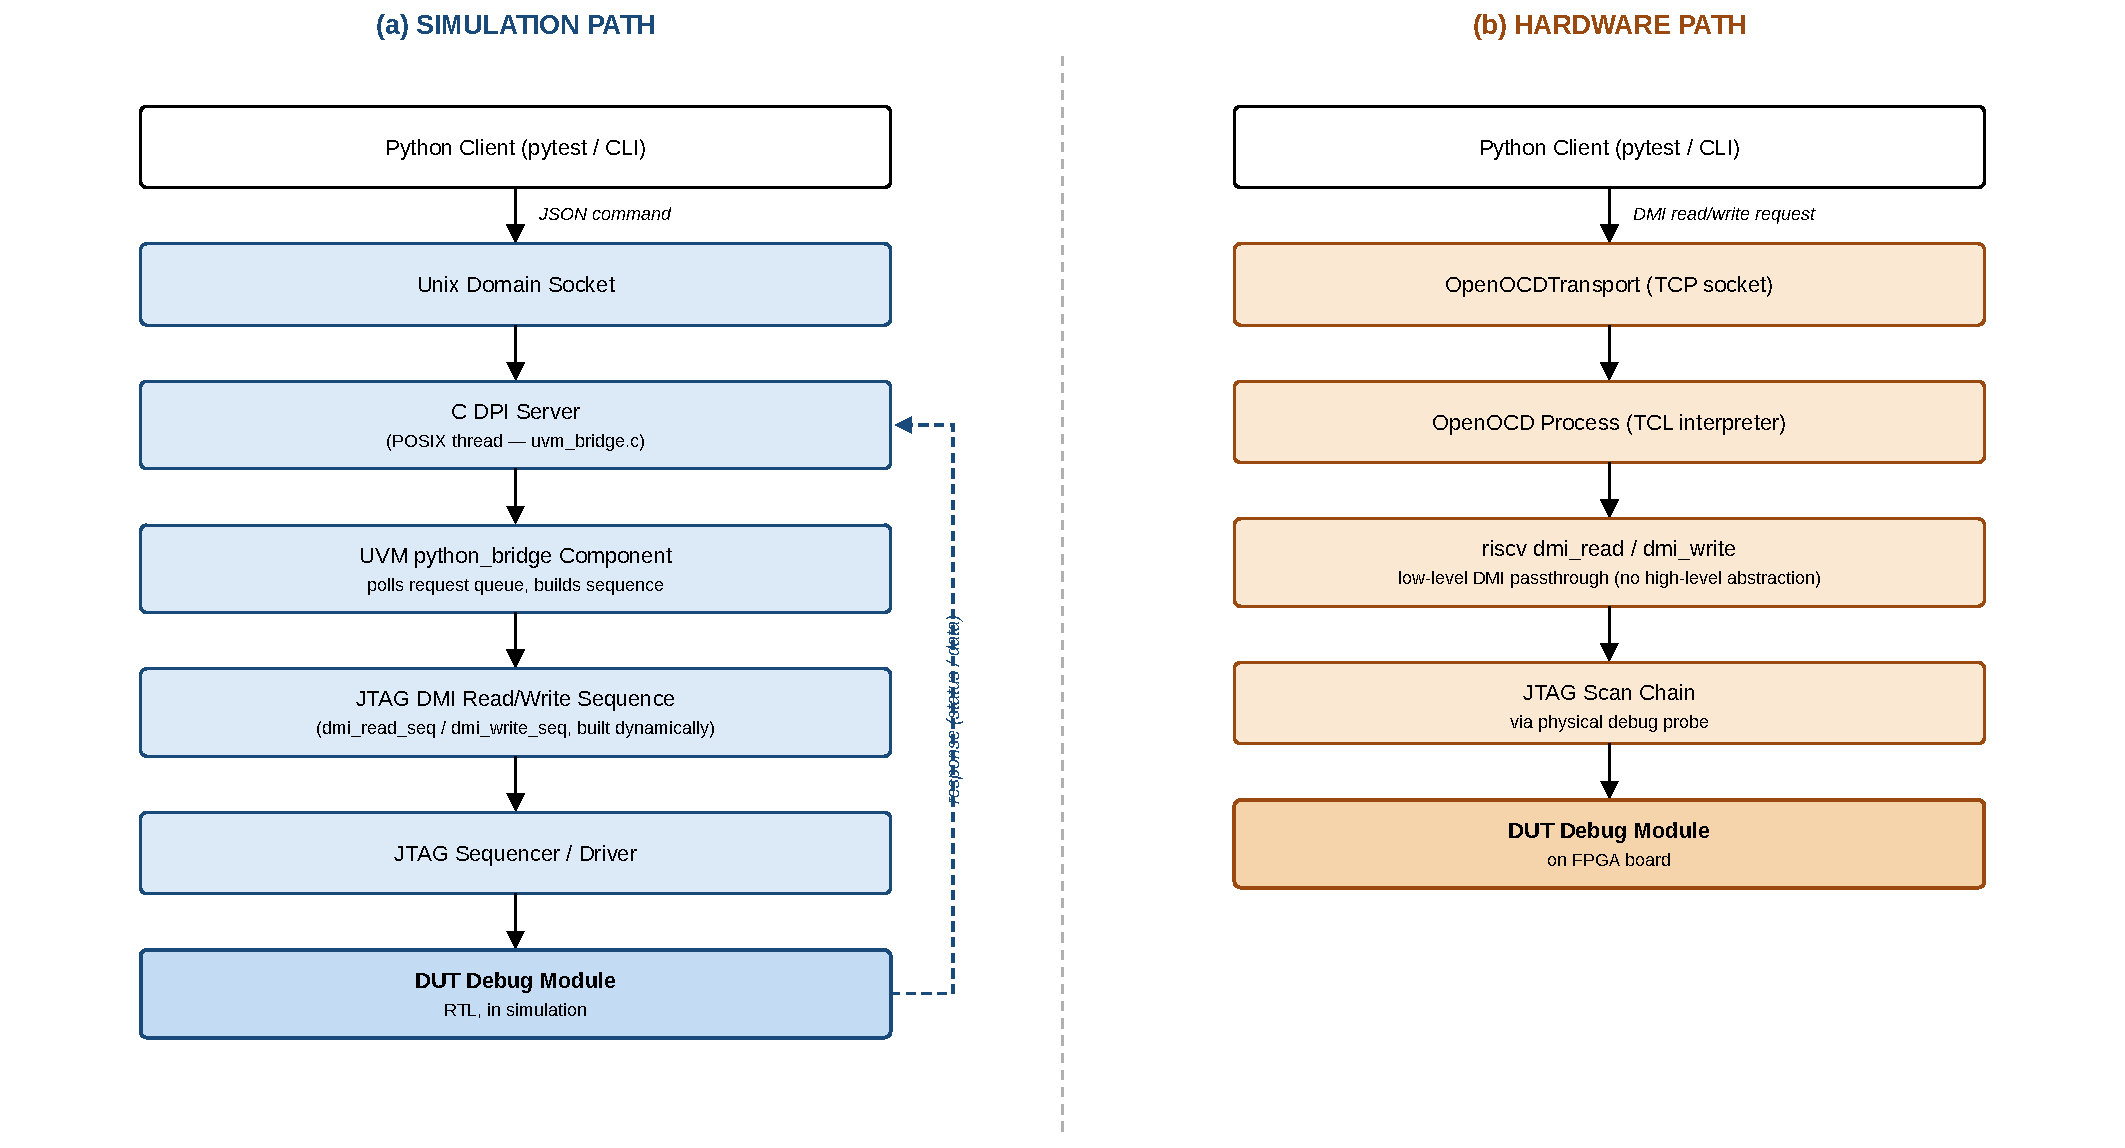
\includegraphics[width=\textwidth]{figures/figure2_flows_combined}
\caption{The same DMI request through the simulation path (left) and the hardware path (right); only the stages below the transport interface differ.}
\label{fig:2}
\end{figure*}

Every run is self-checked. A SystemVerilog reference model of the Debug Module's register state, derived from the specification text rather than from the RTL under test, predicts the expected response to each DMI transaction; a checker compares that prediction against what the RTL returned. Covergroups sample the same stream. Both the model and the covergroups read a per-DUT configuration file declaring that DUT's implementation-defined fields, so neither contains hardcoded per-DUT branches.

\subsection{Emulation and Post-Silicon Flow}
For hardware targets the framework switches to an OpenOCD transport \cite{b7}, using the RISC-V-specific distribution \cite{b8}. Rather than OpenOCD's high-level commands it issues low-level DMI reads and writes, so OpenOCD acts purely as a protocol translator into JTAG scans. The register operations executed on silicon are therefore the same operations executed in simulation.

\subsection{Batch and Interactive Execution Modes}
The same library is exposed through two modes over either transport. In \textbf{batch} mode a scenario runs start to finish unattended; this is the mode used for every result in Section IV. In \textbf{interactive} mode the framework attaches to a live simulation or board and presents a debugger-style prompt, so an engineer can halt, inspect \texttt{dmstatus}, read a register and decide the next operation while the target stays halted. Both modes call the same command layer over the same interface, so an interactive investigation exercises the code path the regression exercises, and a sequence found interactively during bring-up can be committed as a regression scenario without translation.

\section{Experimental Results}
\subsection{Verification Environment}
The framework was evaluated against two RISC-V cores:

\begin{itemize}
\item \textbf{CVA6}, an application-class 64-bit core, with a debug module fork updated to specification version 1.0. This is the v1.0-compliant target.
\item \textbf{Ibex}, in the Ibex Demo System, with \texttt{pulp-platform/riscv-dbg} unmodified at specification version 0.13.
\end{itemize}

The two \textit{cores} and SoC integrations are unrelated. The two \textit{debug modules} share upstream ancestry but have diverged substantially: across the shared file set, 1102 of 3333 lines differ (33\%), with the register file \texttt{dm\_csrs.sv} and the JTAG DTM \texttt{dmi\_jtag.sv} each roughly half rewritten between the v0.13 baseline and the v1.0 fork. Section IV-E depends on this characterisation and does not overstate it.

Both were simulated in Questa Sim-64. Seventeen scenario configurations per core were executed, each self-checked and instrumented for coverage. All results below come from re-running the complete regression on both cores for this paper.

\subsection{Simulation Results}
Table II reports every scenario under two independent checks. \textit{Txn} counts DMI transactions the scoreboard validated for protocol and response consistency, \textit{Err} those that failed. \textit{Chk} counts register reads compared against the specification-derived reference model, \textit{MM} those that diverged from its prediction.

\begin{table*}[!t]
\caption{Full simulation regression, both DUTs}
\label{tab:II}
\centering
\footnotesize
\begin{tabular}{lp{0.26\textwidth}cccc}
\toprule
Scenario & Debug feature exercised & CVA6 (v1.0) Txn / Err & CVA6 Chk / MM & Ibex (v0.13) Txn / Err & Ibex Chk / MM \\
\midrule
\texttt{discovery} & DM presence, version, \texttt{hartinfo} & 7 / 0 & 3 / 0 & 7 / 0 & 3 / 0 \\
\texttt{dm\_activation} & \texttt{dmactive} reset and activation & 18 / 0 & 7 / 0 & 18 / 0 & 7 / 0 \\
\texttt{read\_dmstatus} & Raw \texttt{dmstatus} read & 2 / 0 & 1 / 0 & 2 / 0 & 1 / 0 \\
\texttt{report\_halt\_status} & Halt-status reporting & 11 / 0 & 4 / 0 & 11 / 0 & 4 / 0 \\
\texttt{halt} & Halt request and acknowledgment & 42 / 0 & 16 / 0 & 36 / 0 & 13 / 0 \\
\texttt{run\_control} & Halt and resume run control & 49 / 0 & 15 / 0 & 49 / 0 & 15 / 0 \\
\texttt{reset\_ctrl} & \texttt{ndmreset} and \texttt{hartreset} & 68 / 0 & 20 / 0 & 66 / 0 & 19 / 0 \\
\texttt{halt\_on\_reset} & Halt-on-reset request & 23 / 0 & 7 / 0 & 23 / 0 & 7 / 0 \\
\texttt{hart\_selection} & \texttt{hartsel} / \texttt{hasel} addressing & 15 / 0 & 4 / 1 & 15 / 0 & 4 / 1 \\
\texttt{gpr\_write} & GPR write and read-back & 33 / 0 & 12 / 0 & 27 / 0 & 9 / 0 \\
\texttt{csr\_access} & CSR access via abstract command & 56 / 0 & 20 / 0 & 48 / 0 & 16 / 0 \\
\texttt{program\_buffer} & Program Buffer execution & 40 / 0 & 14 / 0 & 36 / 0 & 12 / 0 \\
\texttt{single\_step} & Hardware single-step & 156 / 0 & 73 / 0 & 50 / 0 & 18 / 0 \\
\texttt{sw\_breakpoint\_progbuf} & SW breakpoint via Program Buffer & 38 / 0 & 15 / 0 & 30 / 0 & 11 / 0 \\
\texttt{sba} & System Bus Access, 32-bit & 20 / 0 & 6 / 0 & 20 / 0 & 6 / 0 \\
\texttt{trigger} & Trigger module registers & 117 / 0 & 33 / 0 & 117 / 0 & 33 / 0 \\
\texttt{external\_trigger} & Halt-group discovery via \texttt{dmcs2} & 13 / 0 & 4 / 0 & 13 / 0 & 4 / 0 \\
\textbf{Total (17 scenarios)} &  & \textbf{708 / 0} & \textbf{254 / 1} & \textbf{568 / 0} & \textbf{182 / 1} \\
\bottomrule
\end{tabular}
\end{table*}

Every scenario completes on both DUTs. Across 1276 scoreboard-checked transactions there are no protocol errors, and of 436 register values compared against the reference model, 434 match its prediction exactly.

The two divergences are the same divergence, once per DUT: \texttt{dmstatus.allrunning} and \texttt{anyrunning} read 1 for a hart selection that does not exist, where the specification requires the hart to be reported as non-existent. Both return a \texttt{dmstatus} word differing from the prediction in exactly bit 11. The defect sits in the portion of the debug module the two still share and predates the v1.0 fork. It is filed with the RTL owners and deliberately not patched, consistent with treating this work's scope as the stimulus framework rather than the design.

Two entries warrant comment. \texttt{single\_step} checks more state on CVA6 because the v1.0 module exposes additional \texttt{dcsr} fields the scenario polls; the difference is scenario-driven. \texttt{external\_trigger} returns a negative result on both and is reported as such rather than omitted: \texttt{dmcs2} does not exist at v0.13, and although it exists in the v1.0 fork every field reads as tied to zero, so halt groups are genuinely unimplemented on both targets.

Program Buffer execution is a genuine execution proof rather than a register round-trip: the scenario injects \texttt{addi x5, x5, 1; ebreak}, triggers it through \texttt{postexec}, and confirms \texttt{x5 = 1} on real RTL. The software-breakpoint scenario recorded a falsifiable prediction in advance --- that \texttt{dcsr.cause} remains unchanged when \texttt{ebreak} executes on an already-halted hart --- which the run then confirmed.

\subsection{Functional Coverage Closure}
Passing scenarios are a necessary but insufficient bar; the acceptance criterion adopted was complete functional coverage of the external-debug feature set. Each scenario's coverage database is saved separately and merged, so a bin hit by any scenario counts as covered.

\begin{table*}[!t]
\caption{Merged functional coverage, external-debug feature set}
\label{tab:III}
\centering
\footnotesize
\begin{tabular}{llcccc}
\toprule
DUT & Spec version & Scenarios merged & Covergroup types & Bins covered / total & Merged coverage \\
\midrule
CVA6 & 1.0 & 17 & 14 & 150 / 150 & \textbf{100.00\%} \\
Ibex & 0.13 & 17 & 14 & 149 / 149 & \textbf{100.00\%} \\
\bottomrule
\end{tabular}
\end{table*}

All 14 covergroups reach 100.00\% individually on both DUTs, so the aggregate is not concealing a weak group. Figure 3 shows how closure was reached, and the shape of that curve carries the more useful result.

\begin{figure*}[!t]
\centering
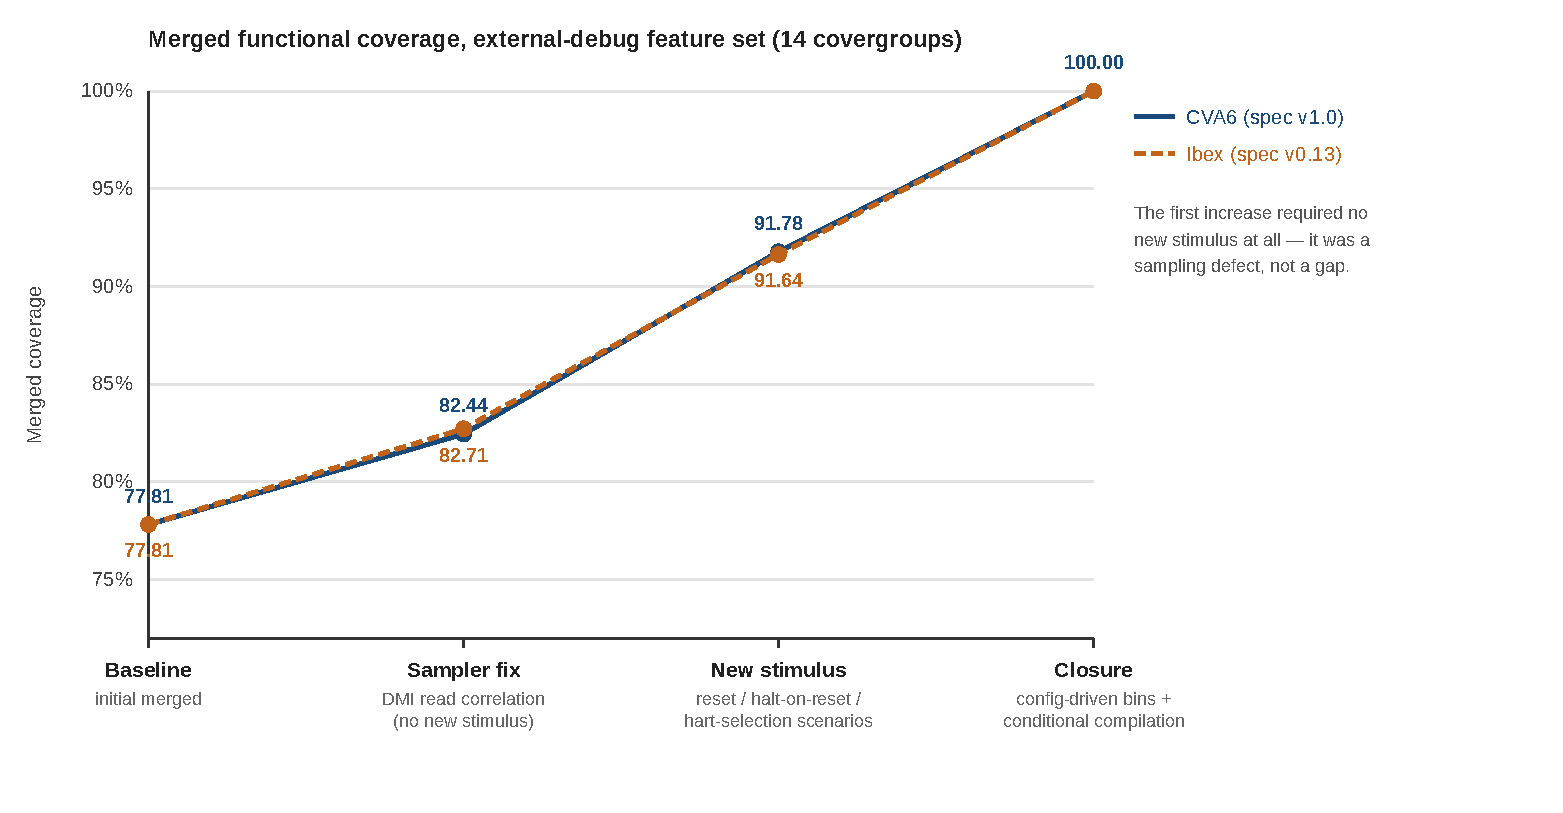
\includegraphics[width=\textwidth]{figures/figure4_coverage_closure}
\caption{Functional coverage closure, annotated with the change responsible for each increase. The first step required no new stimulus at all.}
\label{fig:3}
\end{figure*}

A 100\% figure is only meaningful alongside its denominator. Bins were excluded only where a specific RTL construct makes them unreachable on the integrations under test, each with a citation to that construct: \texttt{allunavail}/\texttt{anyunavail} (the availability input is tied to zero in both SoC integrations), and \texttt{hasresethaltreq} (hardcoded to zero in both debug-module configurations). One bin required genuine conditional compilation rather than exclusion --- \texttt{ndmresetpending} has two independently reachable values at v1.0 and none at v0.13, and a runtime ``unreachable sentinel'' does not remove a bin from the denominator, since only the \texttt{ignore\_bins} keyword does and it is fixed at elaboration. That single bin is the entire difference between the two denominators in Table III.

Two methodological findings generalise. First, covergroups must be \textbf{configuration-driven rather than hardcoded per DUT}: the covergroup file reads the same per-DUT declaration the reference model reads, so each DUT demands only the bins it actually declares. Second, \textbf{a covergroup at a plausible but low percentage is more often a sampling defect than a stimulus gap} --- the first increase in Figure 3, from 77.81\% to 82.44\% on both DUTs, came entirely from correcting a sampler that correlated each DMI read response with the wrong transaction, one level of pipelining the sampler had not accounted for. No stimulus was written. A clean 0\% indicates missing stimulus; an implausibly specific intermediate percentage indicates a correlation bug, and is worth ruling out first.

\subsection{Cross-Platform Reuse, Measured}
The framework's central claim is that a scenario written once runs everywhere. To test it rather than assert it, the complete Ibex scenario set was executed on an Arty A7 board carrying the Ibex Demo System, over the OpenOCD transport and a physical JTAG probe, and the two invocations were then compared file by file.

\begin{table*}[!t]
\caption{Stimulus reuse between simulation and FPGA hardware}
\label{tab:IV}
\centering
\footnotesize
\begin{tabular}{p{0.44\textwidth}p{0.46\textwidth}}
\toprule
Property & Measured \\
\midrule
Scenarios executed on both simulation and hardware & 17 of 17 \\
Scenarios whose stimulus entry point is identical across targets & 17 of 17 \\
Stimulus files / lines of Python & 19 / 2259 \\
Transport-conditional branches in the stimulus layer & \textbf{0} \\
Configuration keys differing between targets & \texttt{transport} and its connection parameters \\
Other per-target differences & 1 (a memory address, in one scenario) \\
SystemVerilog required by the framework, total & \textbf{120 lines, 3 sequences} \\
Artifacts to keep synchronised per new scenario & 1 (versus 2 for a UVM sequence plus an OpenOCD script) \\
\bottomrule
\end{tabular}
\end{table*}

The stimulus layer contains no \texttt{if transport == ...} branch, no hardware flag, and no OpenOCD-specific path anywhere in 2259 lines. The complete per-target delta is declarative. One honest exception: the \texttt{halt} scenario additionally parameterises a memory address, \texttt{0x80000000} in simulation and \texttt{0x00100000} on the board, because the two targets have different memory maps. That is data in configuration, not logic in stimulus, which is the distinction the architecture is built on.

The last two rows are the framework's answer to testbench complexity, and they are measurements rather than estimates. The entire SystemVerilog surface required is three sequences totalling 120 lines --- a DMI read, a DMI write, and a TAP reset. That figure did not change as the scenario count grew from one to seventeen, because scenario logic lives above the seam. The conventional alternative requires a SystemVerilog sequence \textit{and} an OpenOCD script per scenario, in two languages, kept in agreement by hand.

This is what closes the reproduction gap of Section I: a failure observed on the board is described by a file the simulation environment executes directly.

\subsection{What the Methodology Caught, and Its Limits}
Because one stimulus, reference model and checker run against two DUTs, the \textit{distribution} of a failure across them carries diagnostic information before any waveform is opened. Table V records every defect found during the campaign against what that distribution implied.

\begin{table*}[!t]
\caption{Defect localisation via the cross-DUT signal}
\label{tab:V}
\centering
\footnotesize
\begin{tabular}{p{0.19\textwidth}p{0.07\textwidth}p{0.26\textwidth}p{0.37\textwidth}}
\toprule
Symptom & Appeared on & Implied & Actually located in \\
\midrule
\texttt{dmstatus} reads all-zero during halt poll & Both & Shared DV code or common DM lineage & Shared DV: DMI read sequence drained its response in only one of two phases, offsetting every later read by one \\
\texttt{resumeack} mismatches, several hundred & Both & Shared DV code or common DM lineage & Shared DV: model predicted a hart-driven signal synchronously with the triggering write \\
Coverage plateau at 77.81\% & Both & Shared DV code & Shared DV: sampler correlated read data with the wrong transaction \\
\texttt{single\_step} resume timeout & Both & Shared DV code & Shared DV: stimulus reused a resume primitive that polls a state a stepped hart leaves too quickly to observe \\
\texttt{abstractcs.busy} never clears & CVA6 only & CVA6-divergent RTL or CVA6-specific DV & CVA6 RTL: debug-ROM address migration, fixed at source by the RTL owners \\
\texttt{ndmresetpending} mispredicted & Ibex only & Ibex-divergent RTL or a DV assumption about Ibex & Shared DV: model predicted a v1.0-only field regardless of configured version \\
\texttt{allrunning} set for a non-existent hart & Both & Shared DV code or common DM lineage & \textbf{Common DM lineage: a genuine RTL defect in the unchanged 67\%} \\
\bottomrule
\end{tabular}
\end{table*}

The signal is real and it was load-bearing: a symptom on one DUT immediately excluded shared verification code and directed attention to that design, and the reverse held often enough to be useful. But the table also shows the two honest limits of the technique. A symptom on both DUTs does \textbf{not} imply verification code, because the two debug modules share 67\% of their lines --- the last row is a real RTL defect inherited by both, and reading ``appears on both'' as ``must be our bug'' would have misdirected it. And a symptom on one DUT does not imply that DUT's RTL, because verification code can encode a configuration assumption true of only one target, as the \texttt{ndmresetpending} row shows. The correct formulation is weaker than a binary and still useful: the distribution \textit{reorders} the search space, and its value grows with how far the two DUTs have diverged.

Design findings were reported rather than patched. The \texttt{abstractcs.busy} row illustrates the policy paying off: it blocked five scenarios on CVA6 for a period, was reported with transaction-level evidence rather than worked around in stimulus, and was subsequently root-caused and fixed at source by the RTL owners. The CVA6 column of Table II is the result. Had the framework patched around the symptom, the defect would have remained in the RTL.

\subsection{Quantifying the Transport Trade-off}
The OpenOCD transport can also target simulation directly, over the Remote Bit-Bang protocol \cite{b7}: OpenOCD connects to a bit-level JTAG server compiled into the testbench instead of a physical probe, so a scenario can be rehearsed through the actual OpenOCD and JTAG stack before reaching hardware. What does that cost? An identical operation sequence --- activate, halt, then 20 iterations each of register reads and writes, GPR reads and writes via abstract command, and 32-bit System Bus Access reads and writes --- was timed against both transports on the same running simulation of each DUT.

\begin{table*}[!t]
\caption{Direct UVM socket versus OpenOCD with Remote Bit-Bang, measured}
\label{tab:VI}
\centering
\footnotesize
\begin{tabular}{lcccccc}
\toprule
Metric & Ibex direct & Ibex RBB & Ratio & CVA6 direct & CVA6 RBB & Ratio \\
\midrule
Register read (mean) & 2.93 ms & 164.60 ms & 56.1$\times$ & 134.87 ms & 338.50 ms & 2.5$\times$ \\
Register write (mean) & 1.60 ms & 164.57 ms & 103.1$\times$ & 70.43 ms & 363.15 ms & 5.2$\times$ \\
GPR read (mean) & 9.41 ms & 493.23 ms & 52.4$\times$ & 472.86 ms & 1.137 s & 2.4$\times$ \\
Memory read, SBA (mean) & 11.63 ms & 658.00 ms & 56.6$\times$ & 416.17 ms & 1.292 s & 3.1$\times$ \\
Throughput, full sequence & 144.4 ops/s & 2.3 ops/s & 63.1$\times$ & 3.2 ops/s & 1.1 ops/s & 2.9$\times$ \\
\bottomrule
\end{tabular}
\end{table*}

The direct transport is faster on both, but the gap is not a constant: it is between one and two orders of magnitude larger on Ibex. Comparing \textit{simulated} rather than wall-clock time explains why. A register read consumes essentially the same simulated time on both DUTs, 2.3 to 4.0 $\mu$s, so the Remote Bit-Bang path performs no additional simulated work. What differs is wall-clock cost per simulated microsecond, dominated by CVA6 being a far larger design to evaluate each clock edge. Remote Bit-Bang adds a roughly fixed wall-clock cost per JTAG bit, one TCP round trip: +161.7 ms on Ibex's register read against +203.6 ms on CVA6's --- similar in absolute terms despite very different baselines. That fixed cost is a large fraction of Ibex's small per-operation time and a small fraction of CVA6's large one. The generalisable result is that \textbf{Remote Bit-Bang overhead scales with how thin the direct simulation path already is, not with a fixed multiplier}, which argues for measuring this trade-off per DUT rather than assuming a uniform portability tax.

The practical recommendation follows: keep the direct transport as the default for scenario development and coverage regression, and reserve OpenOCD with Remote Bit-Bang for what only it validates --- the external OpenOCD and JTAG stack itself --- where the cost is acceptable at the far lower iteration counts such a check requires.

\section{Limitations and Threats to Validity}
We state the boundaries of these results explicitly.

\textbf{Single-hart only.} Every result is single-hart. Halt and resume groups are unverified because both DUTs leave \texttt{dmcs2} unimplemented, and multi-hart scenarios need a second hart, which for an execution-based debug module is a substantially larger change than a register addition. We therefore make \textbf{no claim about scalability in hart count}. The scalability we do observe is in scenario count: the SystemVerilog surface stayed at 120 lines while scenarios grew to 17 (Table IV).

\textbf{Vendor independence is claimed only where measured.} The framework was exercised across two DUTs from unrelated projects, two debug-module specification versions, and two transports. It was \textbf{not} evaluated on a second simulator or a second FPGA board, so we claim independence at the DUT and transport level and explicitly not at the tool level.

\textbf{Directed, not random.} Scenario selection is directed and traceable to the test plan of Section III-B. This bounds the state space reached compared with random approaches such as \cite{b2}; the campaign nonetheless surfaced the defects in Table V. Layering random generation above the transport seam is future work.

\textbf{Cross-DUT diagnosis is a heuristic, not a proof.} Section IV-E characterises its two failure modes concretely.

\textbf{Coverage is of the model we built.} 100.00\% is against 14 covergroups over the external-debug feature set, with exclusions itemised in Section IV-C. It is not a claim of exhaustive verification, and native-debug paths are outside the model entirely.

\textbf{Measurement caveat.} CVA6 simulates with the design optimizer disabled, a constraint predating this work: enabling it crashes the optimizer on vendored floating-point RTL, independently of this framework. Ibex runs optimised. We do not claim to know CVA6's optimised direct-path latency; the run was attempted and the tool fault is reported in place of an estimated number. Since Remote Bit-Bang's added cost tracks socket round-trip time rather than RTL evaluation, an optimised CVA6 run would lower the direct-path latency without lowering the added cost comparably, so the CVA6 ratios in Table VI should be read as a lower bound.

\textbf{Self-evaluation.} The framework was evaluated by its authors on their own DUTs. To support independent checking, every result derives from committed configurations and recorded logs in the project repository, and both regressions were re-run in full for this paper.

\section{Conclusion and Future Work}
This paper presented a dual-transport Python framework that narrows the gap between pre-silicon and post-silicon debug verification. A scenario is written once against a debug-protocol command layer and executed unmodified against either a UVM simulation or physical silicon.

On two RISC-V cores with different debug-module specification versions, 17 specification-traceable scenarios per core run against real RTL, self-checked transaction by transaction against a specification-derived reference model, with 1276 transactions and no protocol errors. Both cores reach 100.00\% merged functional coverage across 14 covergroups. The complete Ibex scenario set then runs on an Arty A7 board with no change to any stimulus file, a property measured rather than asserted: zero transport-conditional branches in 2259 lines, with the entire per-target delta declarative.

Three results bear on methodology beyond this framework. Running one stimulus library across two DUTs turns the distribution of a failure into a localisation signal --- useful, and bounded in the two specific ways Section IV-E documents. A covergroup at a plausible but low percentage is more often a sampling defect than a stimulus gap. And the portability of an OpenOCD transport is not free, with an overhead that scales inversely with how thin the direct path already is.

The contribution is deliberately narrow. It is not that a transactor can drive hardware from a high-level language, which is established, but that placing the seam at the pre/post-silicon boundary for a protocol whose toolchains are maintained by different teams removes an organisational barrier as well as a technical one, and yields a shared reference model and a differential diagnostic that neither environment provides alone.

\textbf{Future work.} (1) Bring up CVA6 emulation on a Genesys2 board so the hardware evidence covers both cores. (2) Resolve the hart-selection finding with the RTL owners and re-run. (3) Extend the debug-module IP to support halt and resume groups, the one feature area excluded by scope, enabling multi-hart evaluation. (4) Integrate with PSS along the split argued in Section II-A, generating the activity graph declaratively while retaining this transport layer as the execution backend. (5) Layer random generation of the kind in \cite{b2} above the seam, combining stimulus depth with target portability. (6) Evaluate on a second simulator to extend the vendor-independence claim to the tool level.

\section*{Acknowledgment}
The authors thank their colleagues at 10xEngineers for review of the verification strategy and test plan, and for maintaining the RISC-V debug-module RTL against which this framework was evaluated.

\begin{thebibliography}{00}
\bibitem{b1} RISC-V International, ``RISC-V Debug Specification, Version 1.0-STABLE,'' Dec. 8, 2022. [Online]. Available: \url{https://github.com/riscv/riscv-debug-spec}
\bibitem{b2} S. Mishra, L. Hao, A. Sharma, A. Anjum, L. Franco, S. Roy, and J. Scott, ``Random testcase generation and verification of debug unit for a RISC-V processor core,'' in \textit{Proc. Design and Verification Conference and Exhibition U.S. (DVCon U.S.)}, San Jose, CA, USA, 2023.
\bibitem{b3} Accellera Systems Initiative, ``Portable Test and Stimulus Standard,'' Version 3.0, Aug. 2024. [Online]. Available: \url{https://www.accellera.org/images/downloads/standards/pss/Portable_Test_Stimulus_Standard_v3.0.pdf}
\bibitem{b4} cocotb contributors, ``cocotb: a coroutine-based cosimulation library for writing testbenches in Python.'' [Online]. Available: \url{https://www.cocotb.org}
\bibitem{b5} X. Hua, S. Yaze, J. Zou, E. Lin, Y. Zhao, and P. Wang, ``A UVM and Python co-simulation framework for automated memory controller verification,'' in \textit{Proc. Int. Conf. Signal Processing, Computer Networks and Communications (SPCNC)}, Wuhan, China, 2025, pp. 657--660, doi: 10.1109/SPCNC68200.2025.11406641.
\bibitem{b6} J. Bergeron, \textit{Writing Testbenches: Functional Verification of HDL Models}, 2nd ed. Boston, MA, USA: Springer, 2003.
\bibitem{b7} The OpenOCD Project, ``Open On-Chip Debugger: OpenOCD User's Guide,'' Release 0.12.0+dev, Apr. 27, 2026. [Online]. Available: \url{https://openocd.org/doc/pdf/openocd.pdf}
\bibitem{b8} RISC-V Collab, ``riscv-openocd,'' GitHub repository. [Online]. Available: \url{https://github.com/riscv-collab/riscv-openocd}
\end{thebibliography}

\end{document}
